\chapter{基于生成对抗网络的图像转译方法}
\section{生成对抗网络}
\subsection{生成模型}
生成模型(Generative Model)描述的是这样一类模型:从分布$p_{data}$取样的若干样本构成训练集,经过训练,生成模型可以学习并模拟该概率分布$p_{model}$。有些生成模型的可以通过显式概率分布函数表达出来,而有些通过从分布中采样得到数据等隐式表达。越来越多的情况下,我们需要生成模型$p_{model}$生成以假乱真的高质量目标样本。

实际应用中,主要用到的三种生成模型:一是自回归网络(Auto-Regressive Networks,AR模型)又叫Fully-visible Bayes networks(FVBN);二是变分自动编码器(Variational Autoencoder,VAE);三是生成对抗网络(Generative Adversarial Networks,GANs)。这些模型各有其特点,自回归模型在采样过程中效率较低切不容易为图像提供简单的低维编码,变分自动编码器倾向于生成稍微模糊的样本,生成对抗网络训练难以稳定和优化。

本工作研究内容基于生成对抗网络,后续章节将对生成对抗网络的进行详细分析和论述。


\subsection{生成对抗网络原理}
\begin{figure*}[ht]
    \centering
	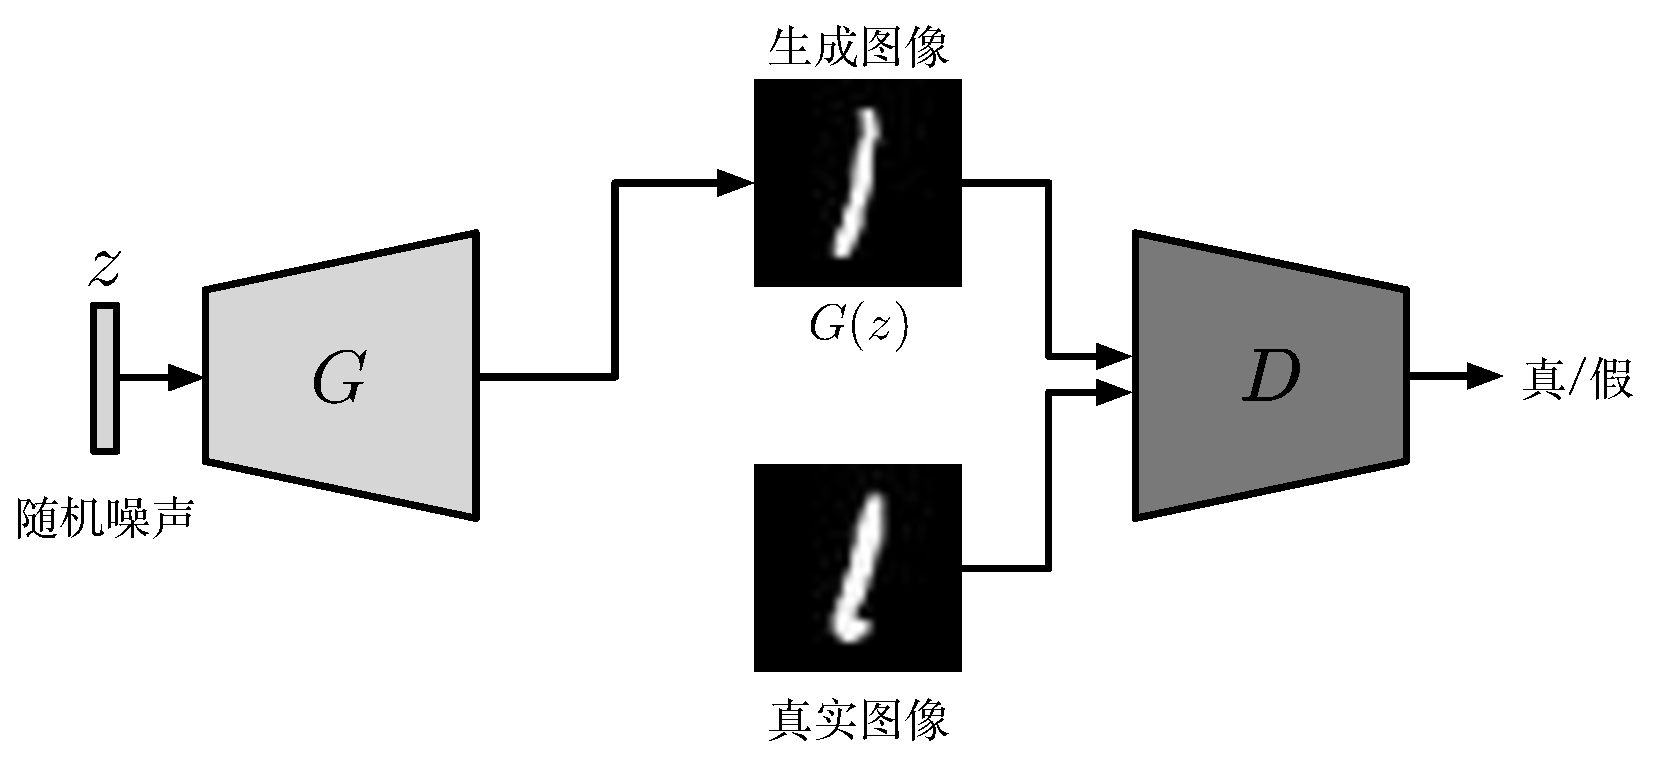
\includegraphics[width=\textwidth]{figures/gan.pdf}
	\caption{生成对抗网络示意图。}
	\label{fig:pic_gan}
\end{figure*}
生成对抗网络是Goodfellow在2014年提出的,生成对抗网络够生成比以往的生成模型更好的合成图像,自此成为最热门的研究领域之一。生成对抗网络的提出采用二人零和博弈思想,两个神经网络在游戏框架下相互博弈,不断彼此优化。
生成对抗网络(GAN)网络结构如图~\ref{fig:pic_gan}所示。由两个彼此独立的神经网络组成:一个生成器(Generator),输入随机噪声向量$z$,输出合成数结果据$G(z)$;一个判别器(Discriminator),输入真实数据$x$或者合成数据结果$G(z)$,判别器试图区分真实数据和合成数据。

% GAN 目标函数
% \mathbf{V}(D,G)  = 
\begin{equation}
\label{equ:equ_gan}
\mathop{min} \limits_{G} \mathop{max} \limits_{D} \mathbb{E}_{x \sim p_{data}(x)}[\log D(x)] + \mathbb{E}_{z \sim p_{z}(z)}[log(1-D(G(z)]
\end{equation}

在训练过程中,生成器和判别器分别单独交替训练,目标函数如式~\ref{equ:equ_gan}所示。优化生成器时判别器固定,生成样本当作真实数据优化,$\min \limits_{G}$最小化生成样本和真是样本之间的差异;优化判别器时固定生成器,把生成样本当作虚假数据进行处理,$\max \limits_{D}$尽可能的让判别器最大化的判别出样本来自真实数据还是生成数据。这是博弈得以进行的关键之处,理想情况下生成分布会拟合于真实分布。

生成对抗网络相比较于之前的生成模型的优势有两点。一是因为不依赖任何先验假设,而传统的方法会假设数据服从某一分布,然后用极大似然去估计分布;二是生成类似真实样本的方法简单,直接利用生成器前向传播进行生成。然而,生成对抗网络也有其不可忽视的缺点。训练中有时不收敛,网络不稳定难以训练;模式坍塌问题,生成的缺少多样性的结果。

\section{生成对抗网络问题和发展}
本节将对生成对抗网络发展过程中具有里程碑意义的变种模型进行介绍,主要在创新点针对网络模型和目标函数的改进,以及解决了传统生成对抗网络的问题。
\subsection{cGAN}

\begin{figure*}[ht]
    \centering
	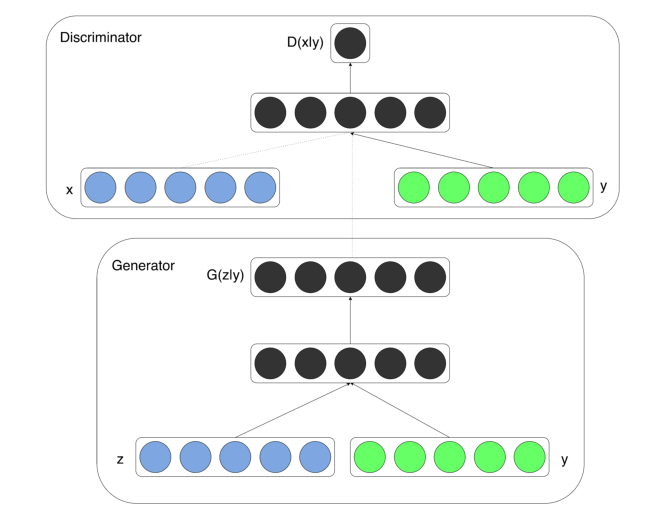
\includegraphics[width=\textwidth]{figures/cgan.pdf}
	\caption{条件生成对抗网络示意图。}
	\label{fig:pic_cgan}
\end{figure*}

原始生成对抗网络不能生成具有特定属性的图像结果,针对这个问题,Mirza等人提出条件生成对抗网络(Conditional Generative Adversarial Nets,cGAN)~\citep{mirza2014conditional}。如图~\ref{fig:pic_cgan}所示,核心创新点在于将属性信息$y$融入生成器$G$和判别器$D$中,属性$y$可以是任何标签信息,例如图像的类别信息或者图像本身等。

% cGAN 目标函数
% \mathbf{V}(D,G)  = 
\begin{equation}
\label{equ:equ_cgan}
\mathop{min} \limits_{G} \mathop{max} \limits_{D} \mathbb{E}_{x \sim p_{data}(x)}[\log D(x|y)] + \mathbb{E}_{z \sim p_{z}(z)}[log(1-D(G(z|y)]
\end{equation}

引入条件$y$后,在GAN基础上的目标函数如式~\ref{equ:equ_cgan}所示。当$y$是特定类别的话,合成结果为特定类别的数据,因此cGAN可以看作从从无监督学习GAN到有监督学习的改进。cGAN生成的图像虽有很多缺陷,譬如图像边缘模糊,生成的图像分辨率太低等,但是它为后续图像风格转换任务中对属性特征的处理提供了方法思路。


\subsection{DCGAN}
从Alex Krizhevsky、Ilya Sutskever和 Geoffrey Hinton创造大型深度卷积神经网络AlexNet\cite{krizhevsky2017imagenet}赢得2012年ImageNet~\cite{deng2009imagenet} 大规模视觉识别挑战赛ILSVRC开始,卷积神经网络(CNN)在计算机视觉领域成功亮相。

\begin{figure*}[ht]
    \centering
	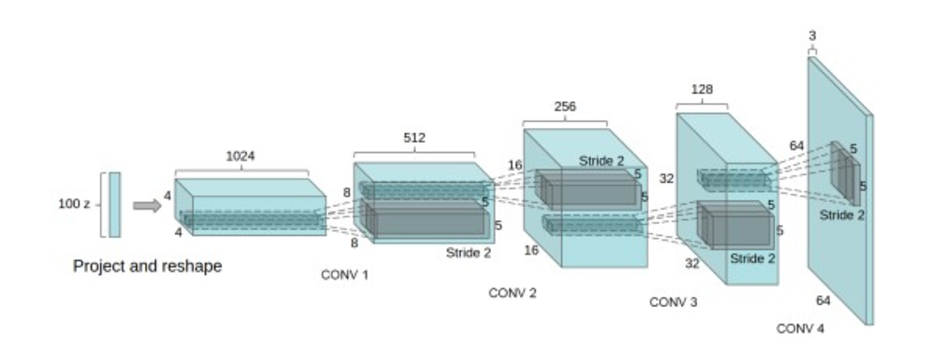
\includegraphics[width=\textwidth]{figures/dcgan.pdf}
	\caption{深度卷积生成对抗网络示意图。}
	\label{fig:pic_dcgan}
\end{figure*}

2016年,Radford等提出了深度卷积生成对抗网络(Deep Convolutional Generative Adverarial Networks, DCGAN)~\cite{radford2015unsupervised},使用深度卷积神经网络代替原始GAN中全链接层的线性感知,将网络拓展至层数更深、参数更多的任务中,进而提高了生成样本的质量和收敛的速度。

深度卷积生成对抗网络对生成对抗网络的模型结构做了一些改变,如图~\ref{fig:pic_dcgan}所示。创新点如下:

(1)在网络结构中取消全链接层,使用全卷积网络。生成器和判别器对称存在,极大的提升了GAN训练稳定和和生成结果质量。

(2)将对抗网络中的池化层取消,使用带步长的卷积层和反卷积层进行上/下采样操作,更好的提取图像特征。

(3)在生成器和判别器中使用批归一化(BatchNorm),为了网络稳定,在生成器输出层和判别器的输入层取消使用批归一化。

(4)生成器中,除了最后一层使用Tanh激活函数外,其余都是ReLU激活函数。

(5)在判别器中,所有层都使用LeakyReLU激活函数,从而防止梯度稀疏。

深度卷积生成对抗网络对生成对抗网络所做的创新,虽然一定程度上稳定了训练,生成较高质量的结果,但是并没有从根本上解决生成对抗网络训练不稳定的问题,在训练过程中仍需要注意生成器和判别器的平衡问题以及模式坍塌问题的出现。

\subsection{LSGAN}
\begin{figure*}[ht]
    \centering
	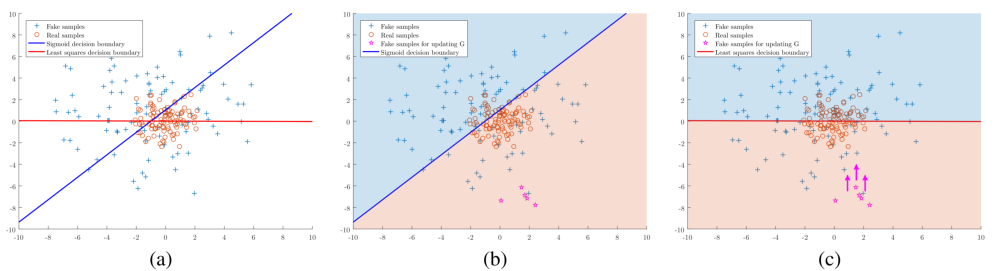
\includegraphics[width=\textwidth]{figures/lsgan.pdf}
	\caption{GAN中Sigmoid决策边界LSGAN最小二乘决策边界图示。}
	\label{fig:pic_lsgan}
\end{figure*}

LSGAN~\cite{mao2017least}针对GAN生成图像质量不高以及训练过程不稳定的问题进行改进,具体来说就是将GAN的目标函数由交叉熵损失换成最小二乘损失。

准确的决策边界会穿过真实数据点,把决策边界当作中介,生成图像结果和真实数据之间的距离可以由生成结果和决策边界之间的距离来反映。如图~\ref{fig:pic_lsgan}所示,蓝色十字形状表示假样本数据,红色空心圆圈是真样本数据,蓝色线条是原始GAN中Sigmoid决策边界,红色线条是LSGAN中最小二乘决策边界。(a)是两个损失函数决策边界对比图。在(b)和(c)中,枚红色五星表示更新生成器过程中的加样本数据。如(b)中所示,橘色是真实数据区域,蓝色是加样本区域。若使用交叉熵作为损失,当交叉熵损失很小时,生成器不会再优化那些被生成器识别为真实图片的生成结果,事实上此时这些生成结果距离决策边界也就是真实数据分布依旧很远,生成器却也不再进行优化。如(c)当损失函数为最小二乘损失时,要想最小化最小二乘损失,生成器必然会将距离决策边界也就是真实数据分布的生成结果拉向决策边界。

LSGAN目标函数定义如式~\ref{equ:equ_lsgan_d}和~\ref{equ:equ_lsgan_g},其中参数设置$a=c=1$,$b=0$
\begin{equation}
\label{equ:equ_lsgan_d}
\min \limits_D \frac{1}{2} \mathbb{E}_{x \sim p_{data}(x)}[(D(x)-b)^2] + \frac{1}{2} \mathbb{E}_{z \sim{p_z(z)}}[D(G(z))-a)^2]
\end{equation}

\begin{equation}
\label{equ:equ_lsgan_g}
\min \limits_G\frac{1}{2}\mathbb{E}_{z \sim{p_z(z)}}[D(G(z))-c)^2]
\end{equation}


\subsection{ACGAN}
\begin{figure*}[ht]
    \centering
	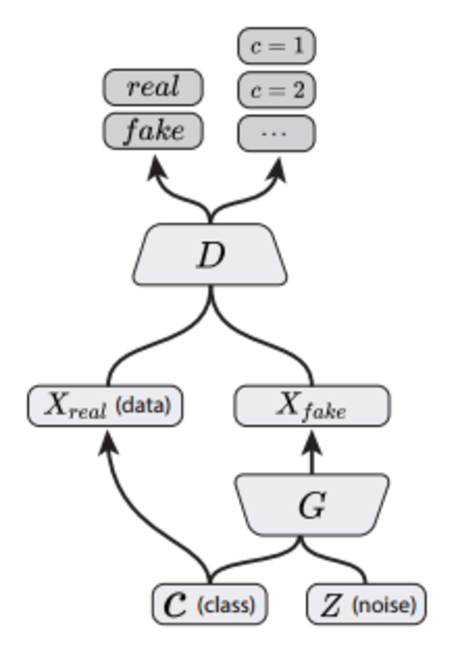
\includegraphics[width=0.4\textwidth]{figures/acgan.pdf}
	\caption{ACGAN结构示意图。}
	\label{fig:pic_acgan}
\end{figure*}

CGAN通过结合标签信息来提高生成数据的质量,ACGAN~\cite{odena2017conditional}除此之外,还通过重建标签信息来提高生成数据的质量。模型结构如图~\ref{fig:pic_acgan}所示,生成器的输入是分类标签和固定的噪声分布,判别器的输出除了指示真假的对抗损失外,还出增加一个辅助分类器判别分类标签,输入的标签当作目标进行反馈,提高判别网络的学习效果。

目标函数包含两个部分:判别真实性的对抗损失$L_S$如式~\ref{equ:equ_acgan_s}和类别判别损失$L_C$如式~\ref{equ:equ_acgan_c}。其核心贡献对于真实图片Xreal和生成器伪造的图片Xfake,辅助分类器应该能够预测它所属的类别。噪声分布$Z$独立于类别标签$C$;判别器训练中试图最大化$L_S+L_C$,而生成器最大化$L_C-L_S$。

\begin{equation}
\label{equ:equ_acgan_s}
L_S = \mathbb{E}[\log P(S = real | X_{real})] + \mathbb{E}[logP(S = fake | X_{fake})]
\end{equation}

\begin{equation}
\label{equ:equ_acgan_c}
L_C = \mathbb{E}[\log P(C = c | X_{real})] + \mathbb{E}[logP(C = c | X_{fake})]
\end{equation}

ACGAN的一个作用就是弥补数据的不足,让计算机拥有了能够模仿现有数据从而生成独特数据的能力,用途相当广泛。

% \subsection{Wasserstein GAN}
% 作者Arjovsky提出Wasserstein GAN(WGAN)~\cite{arjovsky2017wasserstein}在Reddit机器学习频道引起热议。该工作在理论上分析了原始GAN的问题和限制,针对这些问题给出改进算法,主要创新点如下:

% (1)彻底解决了GAN训练不稳定的问题,不需要再平衡生成器和判别器的训练程度。

% (2)基本解决了模式坍塌问题,确保生成样本的多样性。

% (3)Wasserstein距离通过数值指示训练进程,数值越小GAN训练越好,生成质量越高。

% (4)不需要精心设计网络架构,简单的多层全连接网络也可实现。

% 在网络结构上,具体改进为:判别器最后一层去掉sigmoid激活函数,判别器最小化Wasserstein距离,缩小生成分布和真实分布的的Wasserstein距离;生成器和判别器的损失函数不进行$log$计算;每次更新判别器的参数之后,将参数绝对值截断至小于固定参数以满足Lipschitz连续条件;使用非基于动量的优化算法,譬如RMSProp,SGD等适合梯度不稳定的情况。

% 目标函数中,判别器试图最小化式~\ref{equ:equ_wgan_d},其中$m>0$,$[x]^x=max(0,x)$
% % WGAN_D 目标函数
% \begin{equation}
% \label{equ:equ_wgan_g}
% \mathop{min} \limits_{D} \mathbb{E}_{x \sim p(x)}[D(x)] + \mathbb{E}_{z \sim p(z)}[[m-D(G(z))]^+]
% \end{equation}

% 生成器试图最小化式~\ref{equ:equ_wgan_g}
% % WGAN_G 目标函数
% \begin{equation}
% \label{equ:equ_wgan_d}
% \mathop{min} \limits_{G} \mathbb{E}_{z \sim p(z)}[D(G(z)] - \mathbb{E}_{x \sim p(x)}[D(x)]
% \end{equation}

% WGAN有时候也会出现生成样本质量低,难以收敛的问题。

% \subsection{WGAN-GP}
% WGAN-GP~\cite{gulrajani2017improved}是WGAN的改进版,改进了原设计中Lipschitz限制的施加方式,加入梯度惩罚让梯度在后向传播的过程中保持平稳。



\section{基于生成对抗网络的图像转译}
图像翻译旨在通过设计端到端的模型将源域图像转换到目标域图像,通常源域提供图像的内容,目标域提供图像的“风格”(可以是图像属性或图像风格),在源域内容下实现目标域的“风格”化,从而实现源域图像到目标域图像的转换。说的通俗点图像翻译可以是标签图到场景图的转换、线条轮廓到色彩图像转换、图像的风格转换,春夏场景的变换,人脸的属性变换,也可以是白昼交替的转换。只要符合上述端到端转换的任务,都可以通过图像翻译实现。根据训练中是否需要成对图像即源域图像和目标域图像是否一一对应,可以分为成对图像转译和非成对图像转译。、


\subsection{成对图像转译方法}
2017年Isola等人提出pix2pix~\cite{isola2017image},是典型的配对训练图像的图像转译方法。本质上是基于cGAN,将输入图像作为条件,学习从输入图像到输出图像之间的映射,从而得到指定的输出图像。pix2pix等成对图像转译方法可以比较清晰的语义图到真实场景图、灰度图上色、日景到夜景、草图到图像等图像的转换结果。

\begin{figure*}[ht]
    \centering
	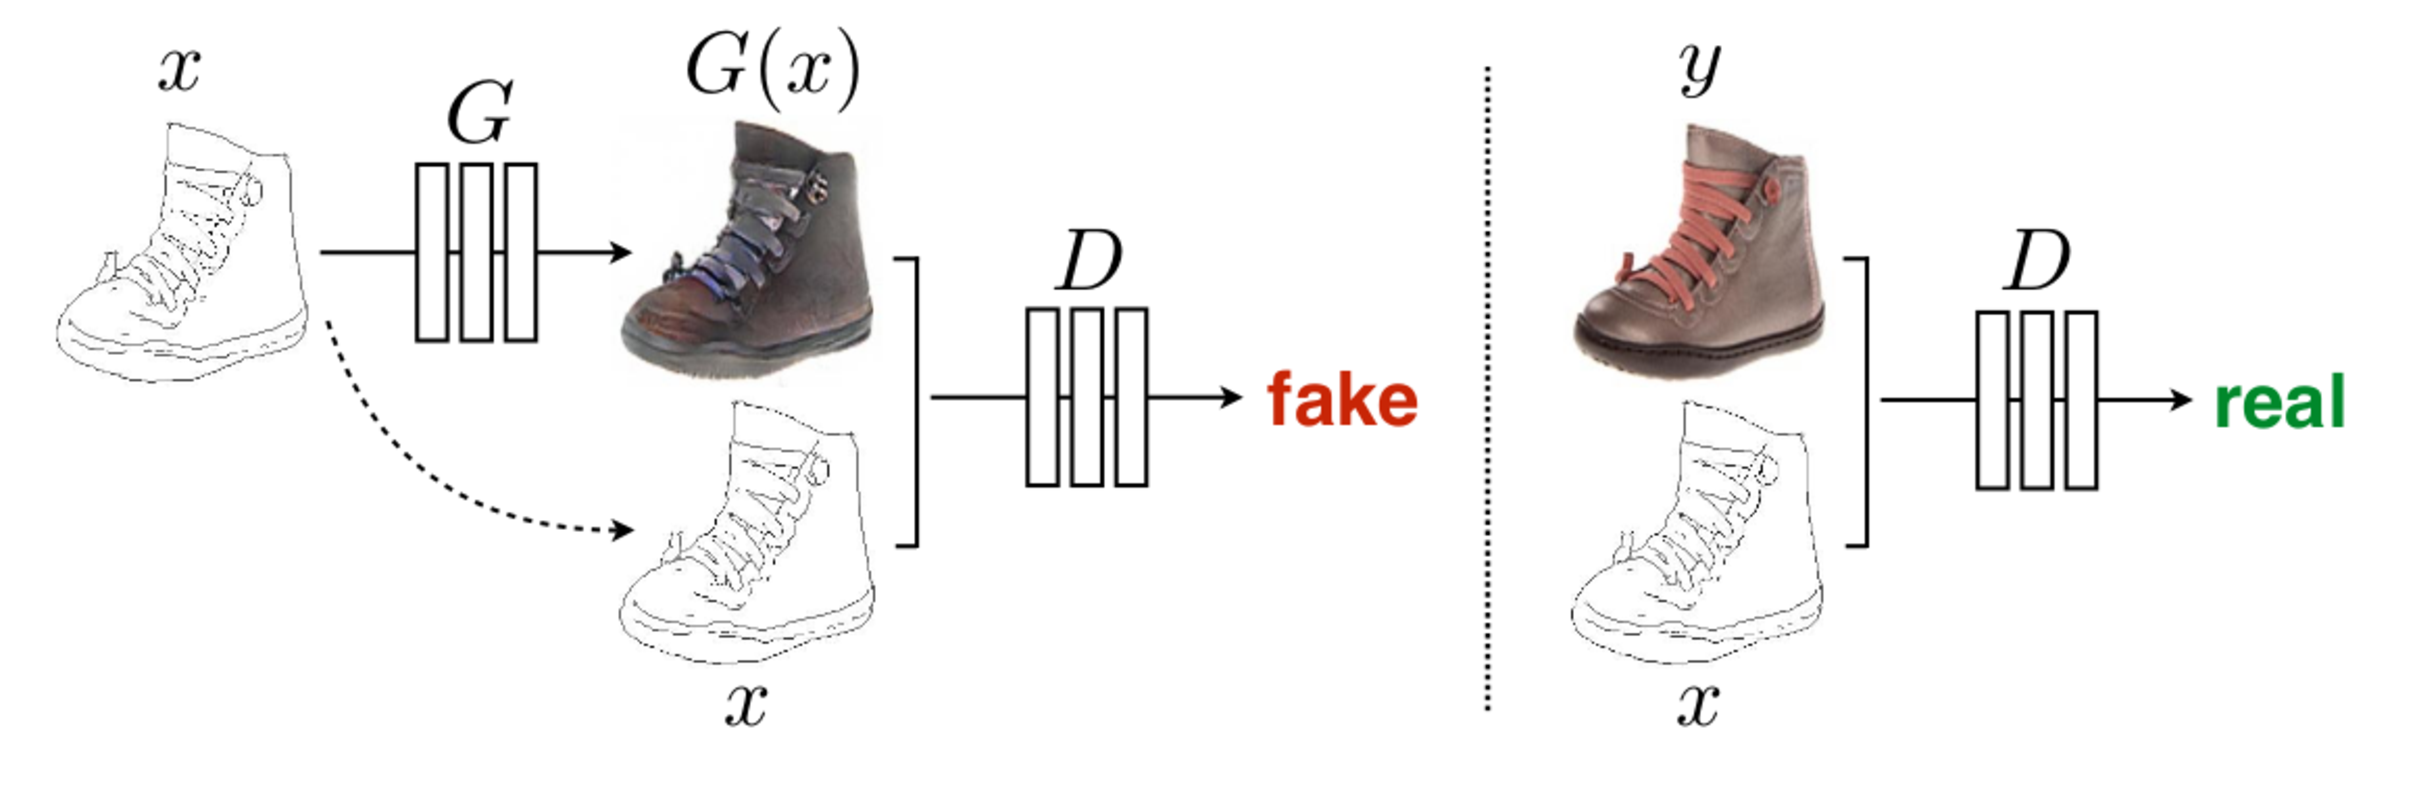
\includegraphics[width=\textwidth]{figures/pix2pix.pdf}
	\caption{pix2pix训练示意图。}
	\label{fig:pix2pix}
\end{figure*}

以草图到图像的转译为例,训练过程如图~\ref{fig:pix2pix}所示。网络结果基于cGAN,将图片$x$作为条件,$y$是跟$x$配对的真实结果,需要输入生成器$G$和判别器$D$中。判别器试图区分合成图像$\{x,G(x)\}$和真实图像$\{x,y\}$,生成器试图生成具有真实性的结果以迷惑判别器。跟无条件GAN不同,pix2pix的生成器和判别器都需要输入条件$x$。

\begin{figure*}[ht]
    \centering
	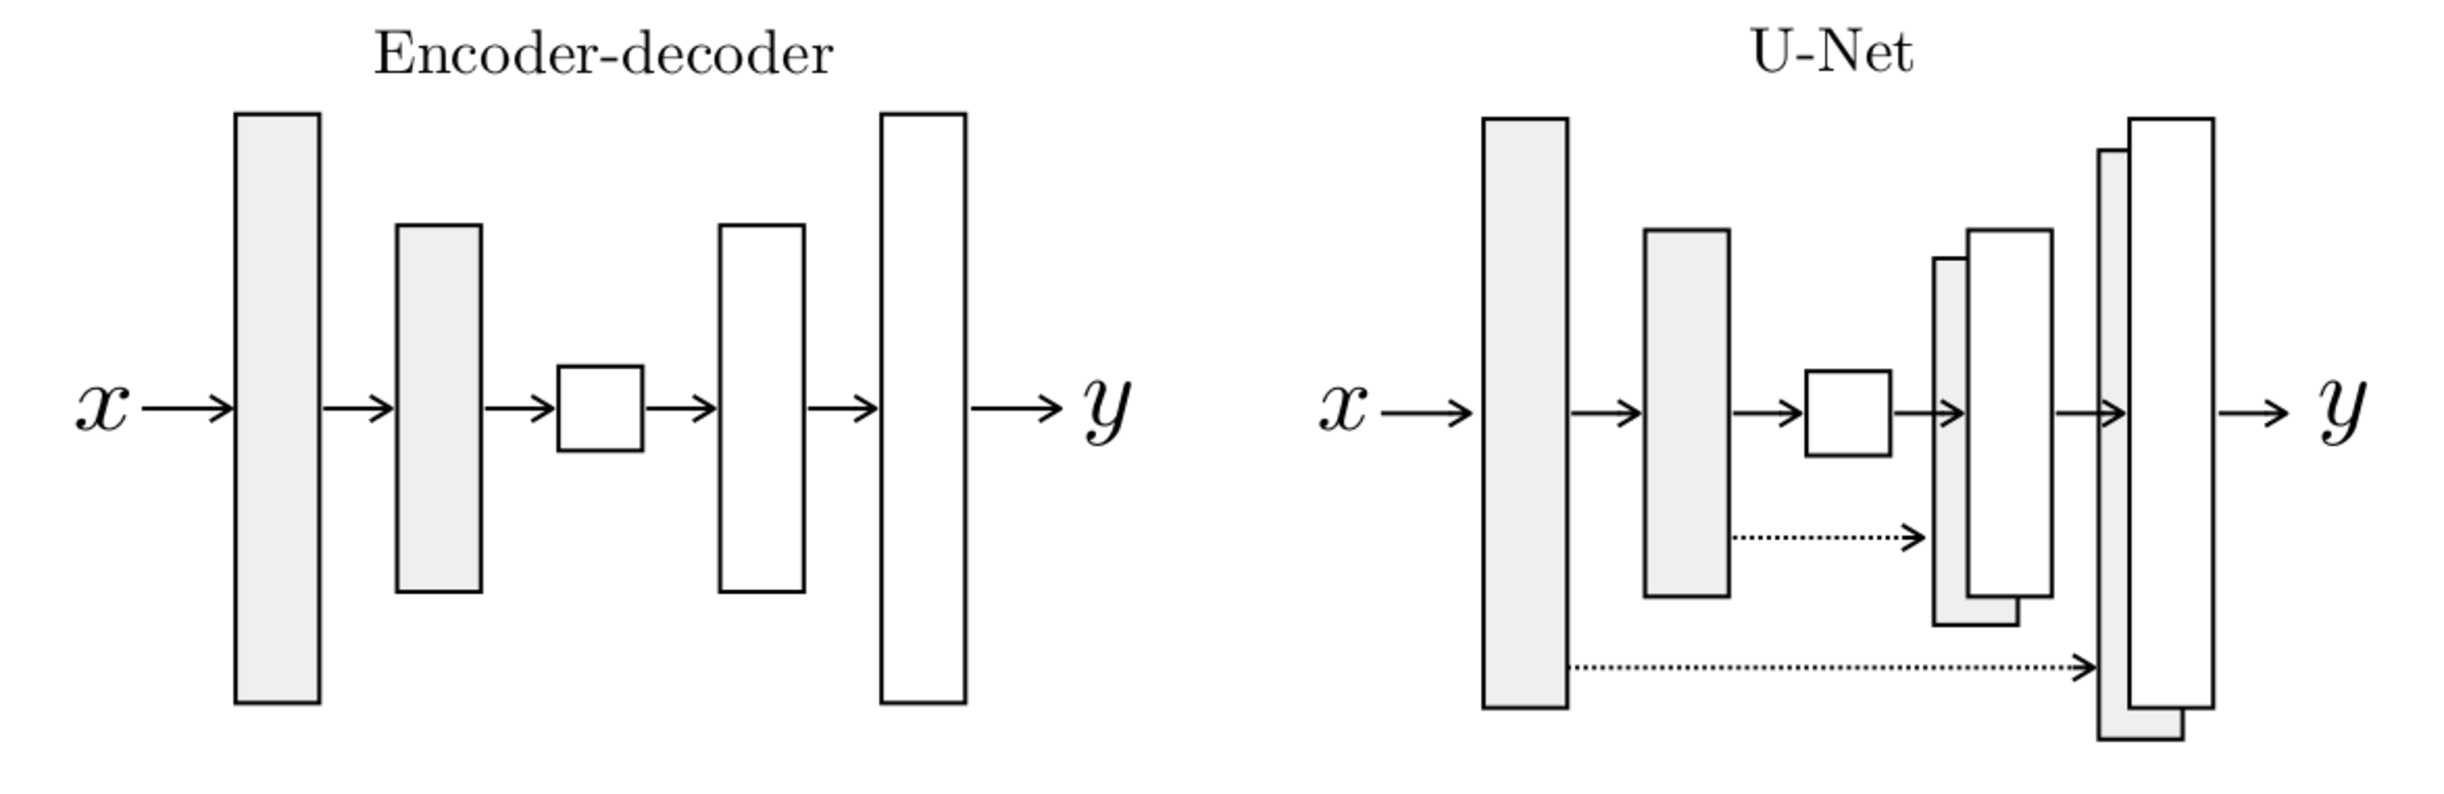
\includegraphics[width=\textwidth]{figures/unet.pdf}
	\caption{pix2pix生成器U-net网络结构示意图。}
	\label{fig:unet}
\end{figure*}

pix2pix的生成器和判别器网络结构在DCGAN的深度卷积的基础上做了一些改进。生成器采用U-Net全卷积结构,跟Encoder-Decoder网络结构先下采样到低维度再上采样到原始分辨率有所区别。如图~\ref{fig:unet}所示,左侧是Encoder-Decoder网络结构,右侧是U-Net~\cite{ronneberger2015u}结构,区别是加入skip-connection,编码过程中对应的特征图和解码之后同样尺寸的特征图按照通道拼接在一起,目的是用来保留不同分辨率下像素级的细节信息。为了更好的对图像局部做判断,判别器利用马尔可夫性的判别器PatchGAN结构。其工作原理是将图像中独立的$N \times N$个patch真假判别,而非将整个图像真假判别,这种设计使得参数更少、运行更快,且能够产生更为锐利的结果。

\begin{equation}
\label{equ:pix2pix_cgan}
L_{cGAN}(G,D) = \mathbb{E}_{x,y}[\log D(x,y)] + \mathbb{E}_{x,z}[\log(1-D(x,G(x,z)))]
\end{equation}

\begin{equation}
\label{equ:pix2pix_l1}
L_{L1}(G) = \mathbb{E}_{x,y,z}[\parallel y-G(x,z) \parallel_1]
\end{equation}

\begin{equation}
\label{equ:pix2pix}
\min \limits_G \max \limits_D L_{cGAN}(G,D) + \lambda L_{L1}(G)
\end{equation}

基于cGAN的目标函数为~\ref{equ:pix2pix_cgan},$L_1$损失为~\ref{equ:pix2pix_l1},总目标函数为~\ref{equ:pix2pix}。$L_1$损失可以恢复图像低频部分让生成图像跟真实训练数据尽量相似,对抗损失额可以恢复图像的高频部分细节。


\subsection{非成对图像转译方法}
很多任务中,由于真实数据限制,我们无法得到成对的源域和目标域图像来进行训练,比如将照片转译成艺术作品风格、人脸转译成漫画风格等源域和目标域图像没有关联性甚至毫不相干的风格转换任务。由此可见,非成对图像转译应用场景更加广泛。

\begin{figure*}[ht]
    \centering
	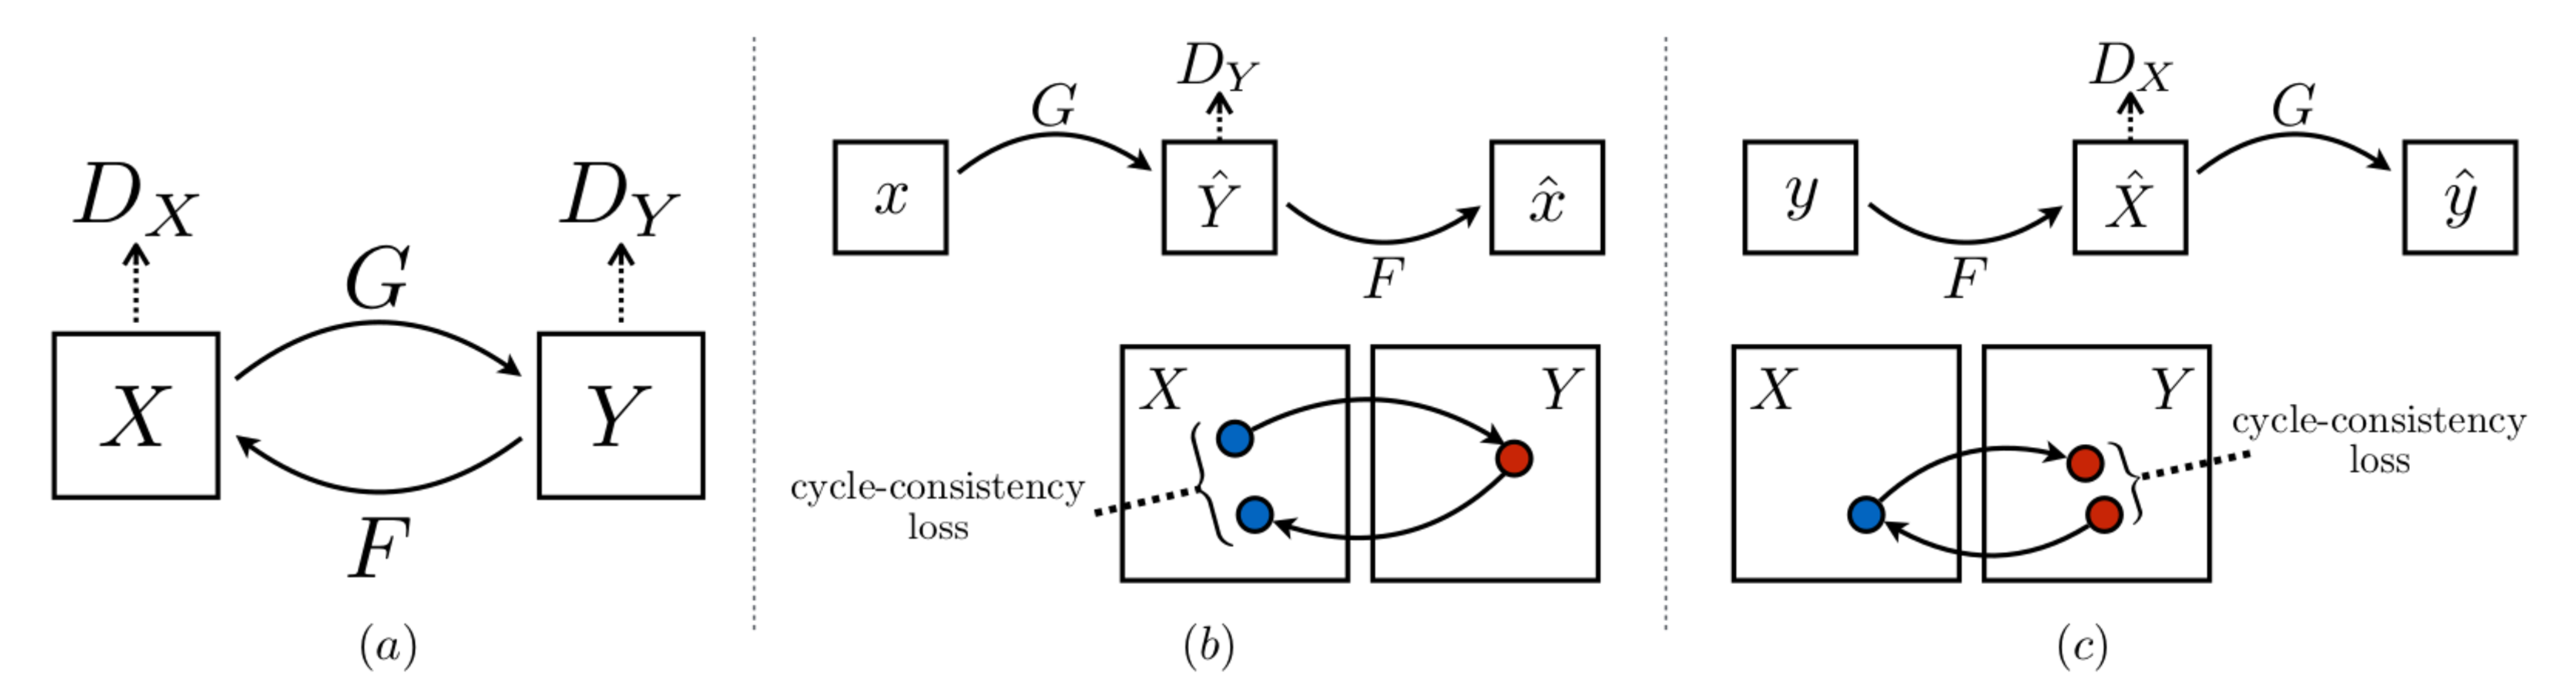
\includegraphics[width=\textwidth]{figures/cyclegan.pdf}
	\caption{CycleGAN网络结构示意图~\cite{zhu2017unpaired}。}
	\label{fig:cyclegan}
\end{figure*}

CycleGAN~\cite{zhu2017unpaired}是一种新颖的无监督循环生成结构,主要思路是训练两对生成器和判别器模型将图像从一个域转换到另一个域,过程中要求循环一致性。实质上,CycleGAN在每个方向上都是单向GAN,共享两个生成器,各自带一个判别器,总共两个生成器两个判别器。网络结构如图~\ref{fig:cyclegan}所示,假设有$X$和$Y$两个域,生成器$G$基于$X$域图像生成$Y$域图像;生成器$F$基于$Y$域图像生成$X$域图像,这两个生成器是相反的过程,通过图~\ref{fig:cyclegan}(b)(c)中的循环一致性损失进行约束。CycleGAN的两个判别器$D_X$和$D_Y$分别用来判断输入$X$和$Y$域的图像真假。因此,CycleGAN可以看作两个GAN的融合,一个GAN由生成器$G$和判别器$D_X$构成,实现从$X$到$Y$域图像的生成和判别;另一个GAN由生成器$F$和判别器$D_Y$构成,实现从$Y$域到$X$域的图像生成和判别,两个网络构成循环过程。

\begin{equation}
\label{equ:cyclegan}
\begin{aligned}
L_{cyc}(F,G,X,Y)= & \mathbb{E}_{x \sim p_{data}(x)}[\parallel G(F(x))-x \parallel_1]\\
& + \mathbb{E}_{y \sim p_{data}(y)}[\parallel G(F(y))-y \parallel_1]
\end{aligned}
\end{equation}

CycleGAN创新提出的循环一致性损失函数如~\ref{equ:cyclegan}所示,映射$ G(F(y)) \approx y$和$ G(F(x)) \approx x$在训练过程中学习到。也就是$X$域图片转译到$Y$域中,还能再逆转回来。生成器$G$对应方向判别器$D_X$和生成器$F$对应方向判别器$D_Y$分别可以定义一个GAN对抗损失,最终目标函数~\ref{equ:cycle_obj}由两个方向上的对抗损失加上循环一致性损失三部分组成。    

\begin{equation}
\label{equ:cycle_obj}
\begin{aligned}
L=L_{GAN}(F,D_Y,X,Y)&+L_{GAN}(G,D_X,X,Y)\\
& + \lambda L_{cyc}(F,G,X,Y)
\end{aligned}
\end{equation}


\subsection{图像多模态转译}
从UNIT~\cite{liu2017unsupervised}以共享潜在空间为假设看成图像求联合概率分布,实现无监督的两个域之间分解表达的图像转译。包括UNIT在内,当时图像转译无论是有监督还是无监督方法,大都是一对一,即输入一张图像只能生成一种风格,缺乏生成结果多样性。比如,同一个场景不同光照条件就是一个模式,不仅仅是白天和黑夜风格,也有傍晚、清晨等风格。在UNIT分解表达学习基础上,MUNIT和DRIT进一步提出多模态图像转译方法。

MUNIT将潜在空间的潜在编码分为内容编码$c$和风格编码$s$。不同域的图像共享内容编码空间$C$而独享风格编码空间$S$。如图~\ref{fig:munit}(a)部分所示,域$X_1$的风格编码空间为$s_1$内容编码空间为$c_1$,域$X_2$的风格编码空间为$s_2$内容编码空间为$c_2$。内容控制图像中低维信息,风格描述图像中高维属性如颜色、纹理、样式等。网络架构清晰,两个编码器$E_1$ $E_2$分别生成域$X_1$和域$X_2$的内容编码和风格编码;两个生成器$G_1$ $G_2$分别生成域$X_1$和域$X_2$的图像结果;两个判别器$D_1$ $D_2$分别判别域$X_1$和域$X_2$的图像真假。

\begin{figure*}[ht]
    \centering
	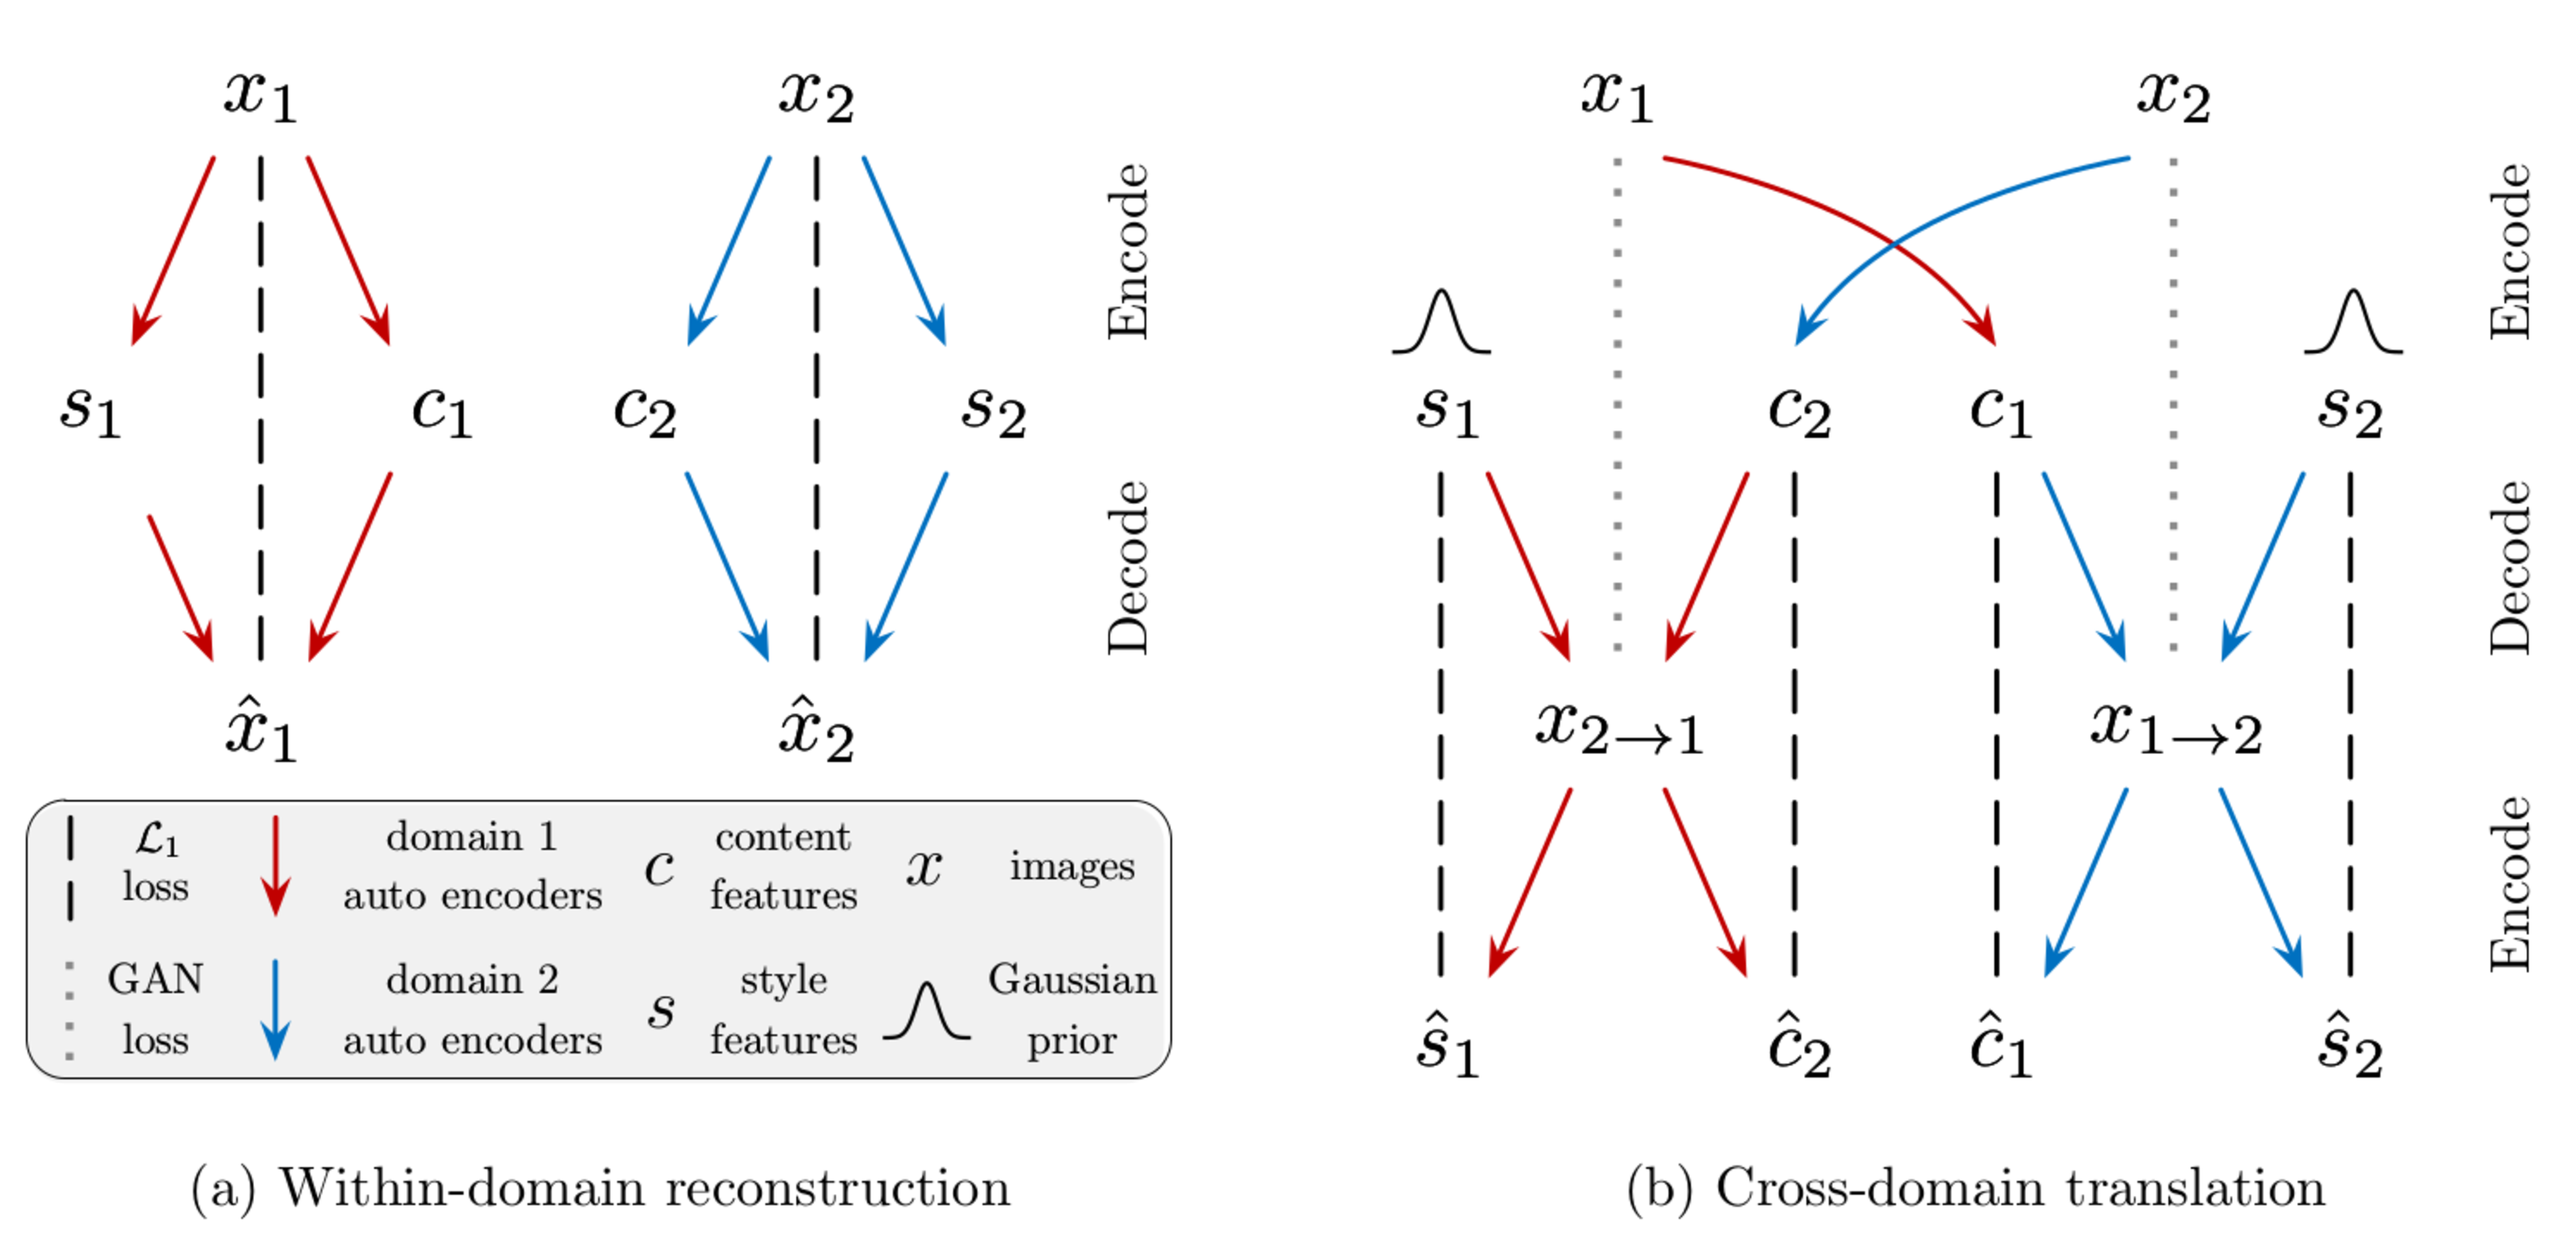
\includegraphics[width=\textwidth]{figures/munit.pdf}
	\caption{MUNIT网络结构示意图~\cite{huang2018multimodal}。}
	\label{fig:munit}
\end{figure*}

整个网络的训练包括两个部分,如图~\ref{fig:munit}(a)所示的域内重建和如图~\ref{fig:munit}(b)所示的跨域转译。

域内重建时,输入图像$x_1 \in X_1$经过编码器$E_1$可以得到内容编码$c_1$和风格编码$s_1$,即$c_1,s_1=E_1(x_1)$,再输入到域$X_1$的生成器$G_1$,形成图像$\hat{x_1}=G_1(c_1,s_1)$。同样的,输入图像$x_2 \in X_2$经过编码器$E_2$可以得到内容编码$c_2$和风格编码$s_2$,即$c_2,s_2=E_2(x_2)$,再输入到域$X_2$的生成器$G_2$,形成图像$\hat{x_2}=G_2(c_2,s_2)$。

跨域转译时,输入图像$x_1 \in X_1$经过编码器$E_1$可以得到内容编码$c_1$和风格编码$s_1$,即$c_1,s_1=E_1(x_1)$,保留内容编码$c_1$与满足正态分布的随机风格编码$s_2$同时输入到生成器$G_2$中,生成具有域$X_2$风格的图像$x_{1 \rightarrow 2}=G(c_1,s_2)$;同样的,输入图像$x_2 \in X_2$经过编码器$E_2$可以得到内容编码$c_2$和风格编码$s_2$,即$c_2,s_2=E_2(x_2)$,保留内容编码$c_2$与满足正态分布的随机风格编码$s_1$同时输入到生成器$G_1$中,生成具有域$X_1$风格的图像$x_{2 \rightarrow 1}=G(c_2,s_1)$。

MUNIT结构包括生成结构和判别结构,生成结构包括编码器和解码器。编码器包括内容编码器和风格编码器,解码器采用AdaIN(Adaptive Instance Normalization)~\cite{huang2017arbitrary}仿射变换将目标域风格转译;判别器使用多尺度判别器~\cite{wang2018high}结构,能帮助实现高分辨率图像的判别。

\begin{equation}
\label{equ:munit_rec_x1}
L_{recon}^{x_1} = \mathbb{E}_{x_1 \sim p(x_1)}[\parallel G_1(E_1^c(x_1),E_1^s(x_1))-x_1\parallel_1]
\end{equation}

% \begin{equation}
% \label{equ:munit_rec_x2}
% L_{recon}^{x_2} = \mathbb{E}_{x_2 \sim p(x_2)}[\parallel G_2(E_2^c(x_2),E_2^s(x_2))-x_2\parallel_1]
% \end{equation}

由此,可以构建重建损失函数包括图像重建损失函数(如式~\ref{equ:munit_rec_x1}),内容重建损失(如式~\ref{equ:munit_rec_c1})和风格重建损失函数(如式~\ref{equ:munit_rec_s2})。

\begin{equation}
\label{equ:munit_rec_c1}
L_{recon}^{c_1} = \mathbb{E}_{c_1 \sim p(c_1), s_2 \sim q(s_2)}[\parallel E_2^c(G_2(c_1,s_2))-c_1\parallel_1]
\end{equation}

% \begin{equation}
% \label{equ:munit_rec_c2}
% L_{recon}^{c_2} = \mathbb{E}_{c_2 \sim p(c_2), s_1 \sim q(s_1)}[\parallel E_1^c(G_1(c_2,s_1))-c_2\parallel_1]
% \end{equation}

% \begin{equation}
% \label{equ:munit_rec_s1}
% L_{recon}^{s_1} = \mathbb{E}_{c_2 \sim p(c_2), s_1 \sim q(s_1)}[\parallel E_1^s(G_1(c_2,s_1))-s_1\parallel_1]
% \end{equation}

\begin{equation}
\label{equ:munit_rec_s2}
L_{recon}^{s_2} = \mathbb{E}_{c_1 \sim p(c_1), s_2 \sim q(s_2)}[\parallel E_2^s(G_2(c_1,s_2))-s_2\parallel_1]
\end{equation}

目标函数(如式~\ref{equ:munit})是对抗损失(如式~\ref{equ:munit_adv})以及重建损失函数之和。
\begin{equation}
\label{equ:munit_adv}
\begin{aligned}
L_{GAN}^{x_2} = & \mathbb{E}_{x_2 \sim p(x_2)}[\log D_2(x_2)] \\
& +\mathbb{E}_{c_1 \sim p(c_1), s_2 \sim q(s_2)}[\log(1-D_2(G_2(c_1,s_2)))]
\end{aligned}
\end{equation}

\begin{equation}
\label{equ:munit}
\begin{aligned}
\min \limits_{E_1,E_2,G_1,G_2} \max \limits_{D_1,D_2} L(E_1,E_2,G_1,G_2,D_1,D_2) & = L_{GAN}^{x_1}+L_{GAN}^{x_2} \\
& +\lambda_x(L_{recon}^{x_1}+L_{recon}^{x_2}) \\
& + \lambda_c(L_{recon}^{c_1}+L_{recon}^{c_2}) \\
& +\lambda_s(L_{recon}^{s_1}+L_{recon}^{s_2})
\end{aligned}
\end{equation}


DRIT~\cite{lee2018diverse}跟MUNIT在思路上完全一致,都是共享内容空间,独享属性/风格空间。网络训练如图~\ref{fig:drit}所示同样由域内重建和跨域转译两个部分组成,跨域转译用来生成交换风格厚的图像,域内重建被编码后的潜在编码。用$X, Y$表示两个域,网络由两个内容编码器$E_{X}^{c}$和$E_{Y}^{c}$和两个属性编码器$E_{X}^{a}$和$E_{Y}^{a}$,两个生成器$G_X$和$G_Y$以及两个判别器$D_X$,$D_Y$组成。

\begin{figure*}[ht]
    \centering
	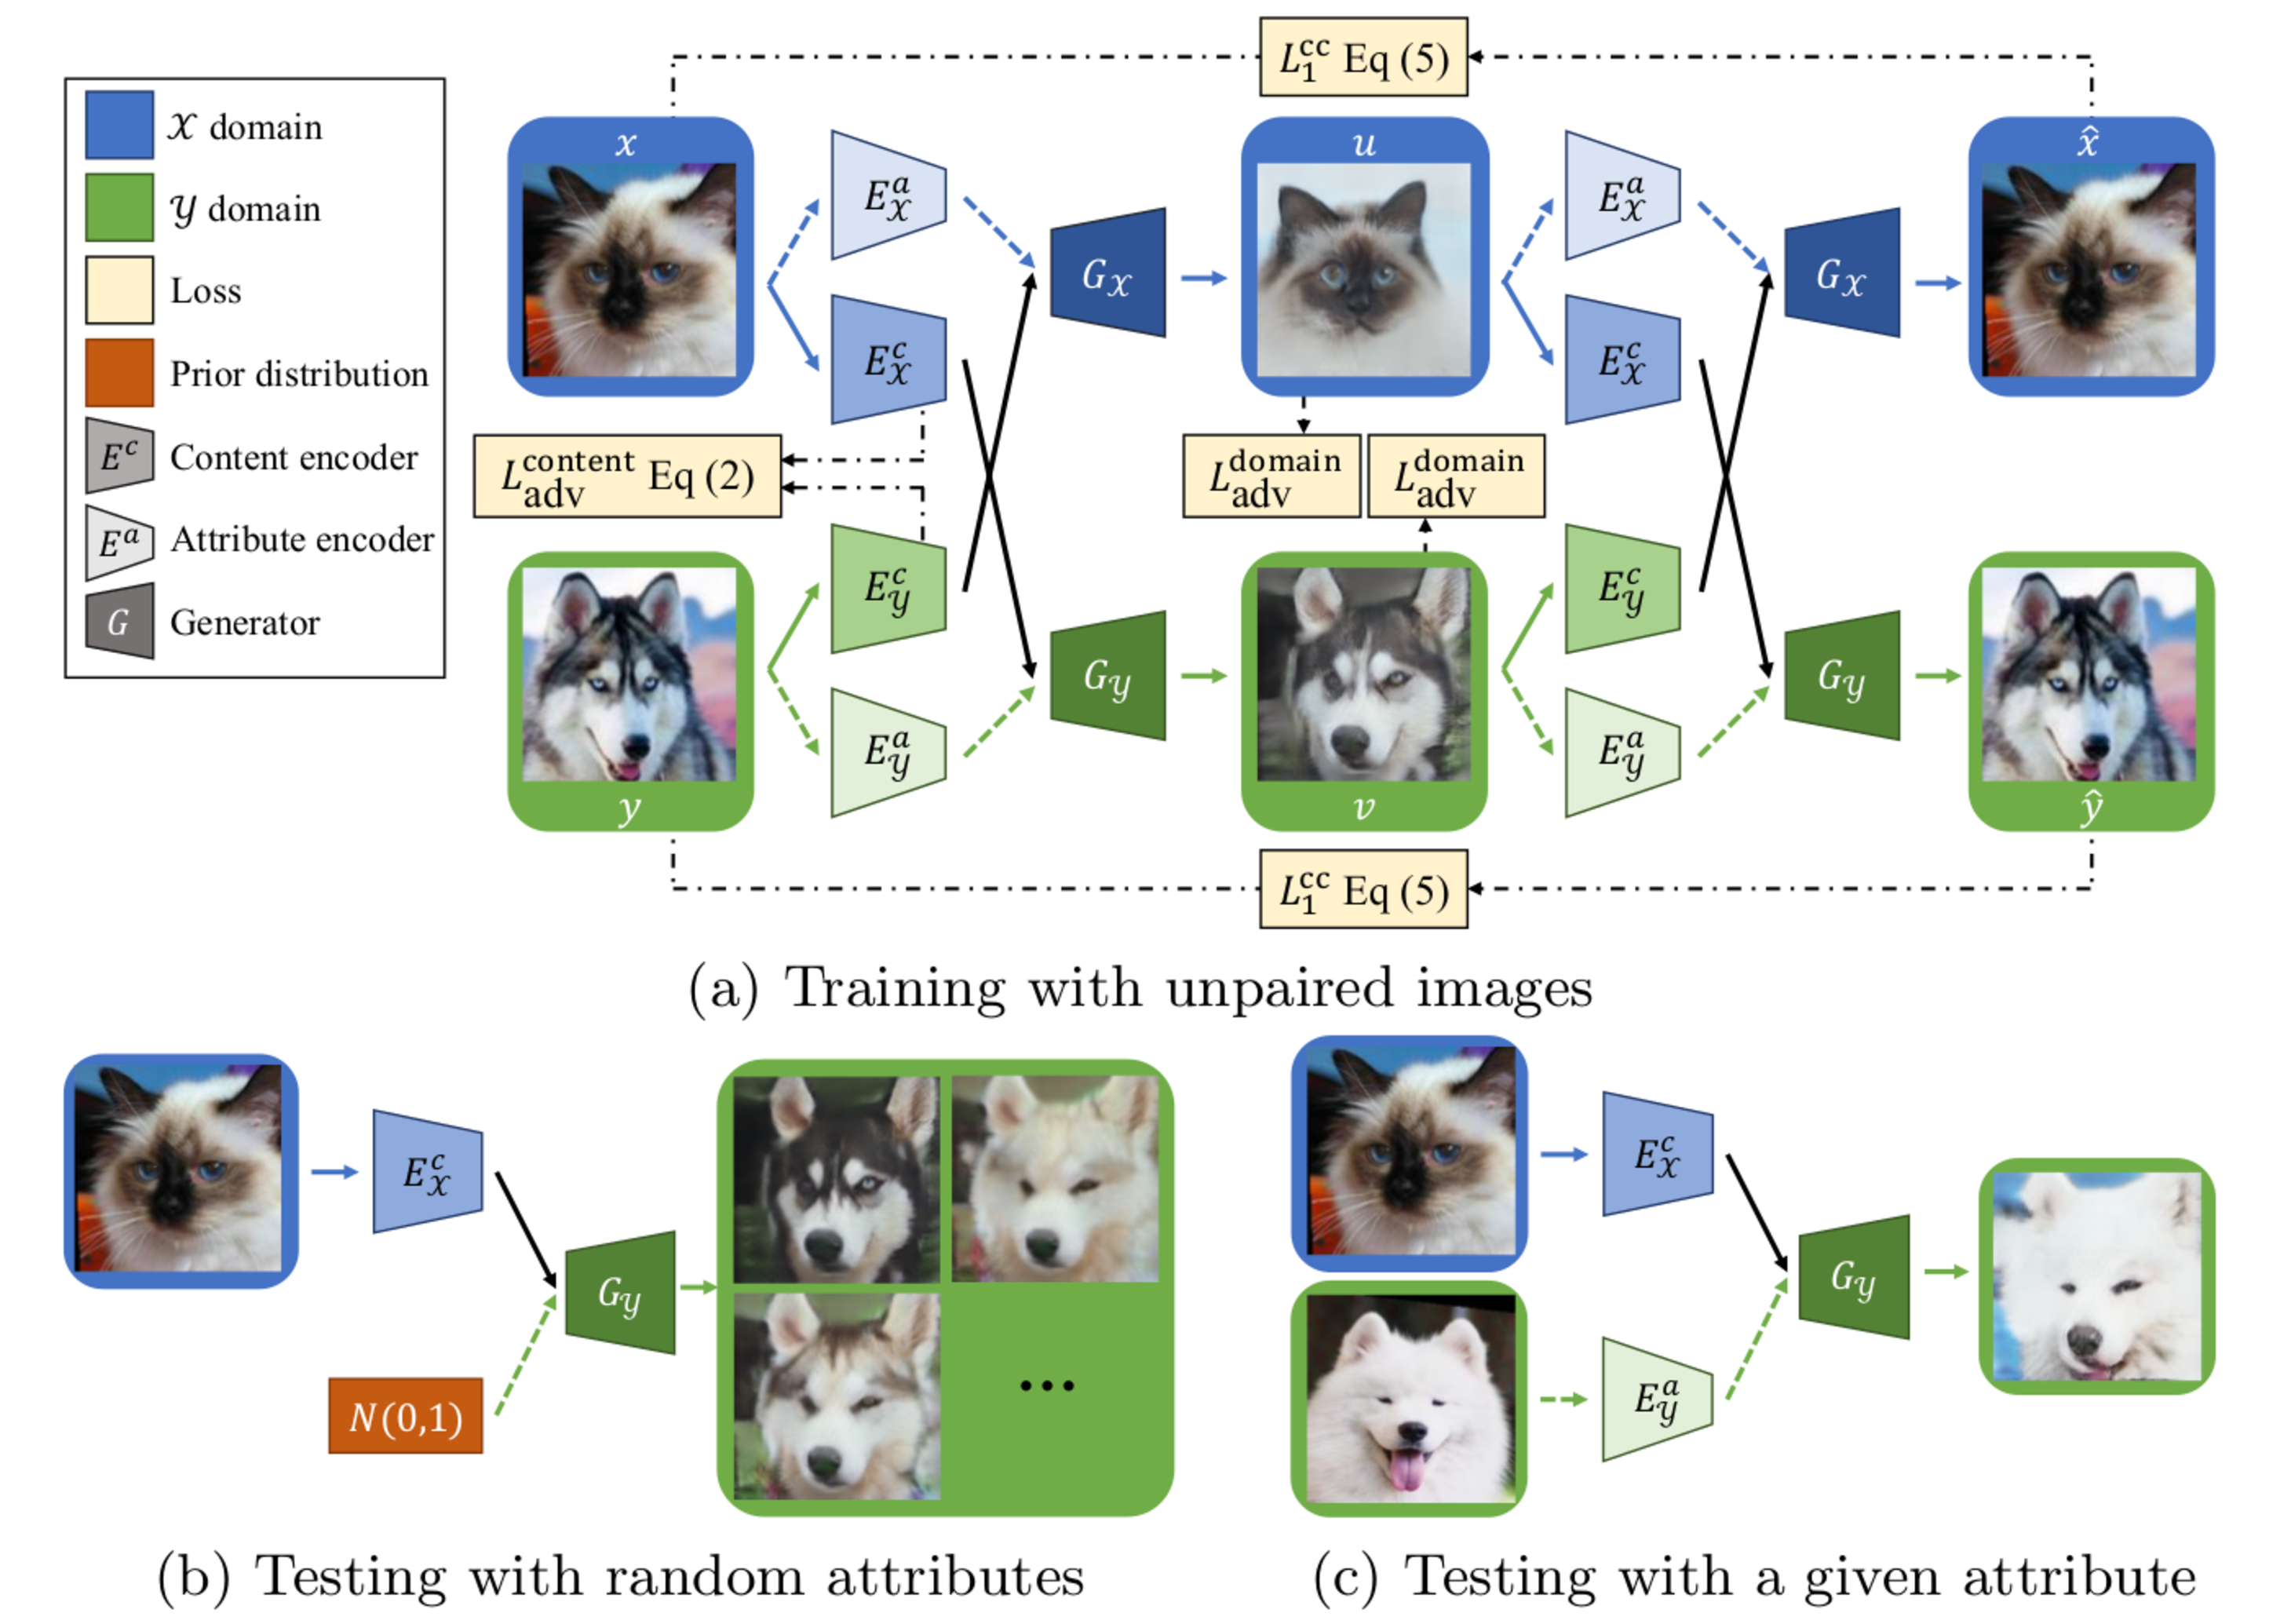
\includegraphics[width=\textwidth]{figures/DRIT.pdf}
	\caption{DRIT训练示意图~\cite{lee2018diverse}。}
	\label{fig:drit}
\end{figure*}

跨域转译和域内重建跟MUNIT一致,在此不再赘述。在内容编码和属性编码结合时,DRIT和MUNIT有一定的差异,MUNIT将风格编码使用AdaIN内嵌到生成器(解码器)的中间层,而DRIT采用共享两个编码器$E_X^c$,$E_Y^c$最后一层和两个生成器$G_X$,$G_Y$第一层的权值。共享权值的情况下,为了区分两个域的编码文中提出使用判别损失~\ref{equ:drit_adv}。

\begin{equation}
\label{equ:drit_adv}
\begin{aligned}
L_{adv}^{content} & = \mathbb{E}_x[\frac{1}{2}\log D^c(E_X^c(x))+\frac{1}{2}\log(1-D^c(E_X^c(x)))] \\
& + \mathbb{E}_y[\frac{1}{2}\log D^c(E_Y^c(y))+\frac{1}{2}\log(1-D^c(E_Y^c(y)))] 
\end{aligned}
\end{equation}

损失函数中也加入CycleGAN中提出的循环一致性损失~\ref{equ:drit_cc},其中$u=G_X(E_Y^c(y),E_X^a(x))$,$v=G_Y(E_X^c(x),E_Y^a(y))$,还有重建损失,对抗损失等。总的目标函数如~\ref{equ:munit}所示。

\begin{equation}
\label{equ:drit_cc}
\begin{aligned}
L_1^{cc}(G_x,G_Y,E_X^c,E_Y^c,E_X^a,E_Y^a) = \mathbb{E}_{x,y}&[\parallel G_X(E_Y^c(v),E_X^a(u))-x \parallel_1 \\
& + \parallel G_Y(E_X^c(u),E_Y^a(v))-y \parallel_1]
\end{aligned}
\end{equation}

\begin{equation}
\label{equ:drit}
\begin{aligned}
\min \limits_{G,E,E^a} \max \limits_{D,D^c} & \lambda_{adv}^{content}L_{adv}^c + \lambda_1^{cc}L_1^{cc} + \lambda_{adv}^{domain}L_{adv}^{domain} \\
& + \lambda_1^{recon}L_1^{recon} + \lambda_1^{latent}L_1^{latent} + \lambda_{KL}L_{KL}
\end{aligned}
\end{equation}

除了MUNIT和DRIT这些经典的多模态转译工作外,近期发表的工作StarGAN v2~\cite{choi2020stargan}是在StarGAN~\cite{choi2018stargan}多域一对一转译任务的基础上,进一步实现了多个域彼之间的多模态转译。DRIT++~\cite{lee2020drit++}则是在DRIT两个域多模态转译任务基础上,进一步实现多域之间转译。越来越多的研究工作,将多模态转译任务拓展至更广泛的应用场景。


\section{本章小结}
本章深入分析介绍了基于生成对抗网络的多模态转译方法。

第一节介绍了生成模型以及各自特点,引入生成对抗网络结构和原理,分析了生成对抗网络的优缺点。

第二节介绍了生成对抗网络的研究历史,详细阐述了在生成对抗网络的发展过程中,针对生成对抗网络中存在的问题进行解决和具有里程碑意义的经典模型。

第三节在前两节铺垫的基础上,引入基于生成对抗网络的多模态转译概念,展示了经典成对图像转译和非成对图像转译经典方法,仔细研究了常用的多模态转译模型以及后续发展的前沿工作。为后续我们基于生成对抗网络的水下图像多模态转译问题奠定理论基础。